\chapter{Configuration Spaces}
% These definitions are presented in Abrams on page 10.
Given a topological space \(X\), the \(n\) point (topological) configuration space of \(X\) is
\(\Conf_n(X) = X^n - \Delta\) where \(\Delta\) is the diagonal in \(X^n\).

Treating a graph \(\Gamma\) as a topological space we can construct the
\(n\) point discretized or combinatorial configuration space \(\DConf_n(\Gamma)\) by 
% this diagonal needs elaboration.
removing a larger diagonal \(\Delta^{\square} = \{(e_1, \ldots, e_n) \mid x_i \cap x_j \neq \emptyset \text{ for some } i \neq j\}\)
from the cubical complex \(\Gamma^n\). Here \((e_1, \cdots, e_n)\) is any \(n\)-tuple of cells in \(\Gamma\).

Abrams in \cite{abrams2000configurationspaces} showed that \(\Conf_n(\Gamma)\) deformation retracts onto \(\DConf_n(\Gamma)\).
\begin{figure}
\centering
\begin{tikzpicture}
    \node (u1) at (2, 2) {\(u_1\)};
    \node (u2) at (4, 2) {\(u_2\)};
    \node (u3) at (3, 1) {\(u_3\)};
    \node (u4) at (3, 0) {\(u_4\)};
    \draw (u1) -- (u3);
    \draw (u2) -- (u3);
    \draw (u4) -- (u3);
\end{tikzpicture}
\caption{The \(Y\)-graph}
\label{fig:ygraph}
\end{figure}
In \cite{abrams2000configurationspaces} Abrams notes that any point in the
\(n\)-point configuration space is in one-to-one correspondence with a
collection of ``tokens'' placed on the graph. In this project, we will a
slightly ``particles'' placed on the graph instead.  Let \(\Gamma\) be the graph
in \ref{fig:ygraph} and consider \(2\) particles placed on \(\Gamma\) at \(u_1\)
and \(u_2\).  As the particle at \(u_1\) moves to \(u_3\), in the topological
configuration space the particle at \(u_2\) is free to simultaneously move to
\(u_3\) as well. However, both particles would not be able to occupy the vertex
\(u_3\) simultaneously.  In the combinatorial configuration space, as the
particle at \(u_1\) moves to \(u_3\), the particle at \(u_2\) can not move at
all since the edges \(u_1 u_3\) and \(u_2 u_3\) intersect at \(u_3\) and points
with coordinates belonging to both edges are thereby removed.

\begin{figure}
\centering
\begin{tikzpicture}
    \node (v1) at (0, 2) {\(v_1\)};
    \node (v2) at (0, 0) {\(v_2\)};
    \draw (v1) -- (v2);
    \node (u1) at (2, 2) {\(u_1\)};
    \node (u2) at (4, 2) {\(u_2\)};
    \node (u3) at (3, 1) {\(u_3\)};
    \node (u4) at (3, 0) {\(u_4\)};
    \draw (u1) -- (u3);
    \draw (u2) -- (u3);
    \draw (u4) -- (u3);
\end{tikzpicture}
\caption{An edge and a \(Y\)-graph}
\label{fig:edgeygraph}
\end{figure}
Consider the graph in figure \ref{fig:edgeygraph} and put particles at \(v_1\) and \(u_2\).
As the particle at \(v_1\) moves to \(v_2\) there are three ways that the particle at \(u_2\) can move.
Since each way that the particle at \(u_2\) can move can be done simultaneously as the movement of the particle at \(v_1\),
the \(1\)-cell corresponding to the movement of the particle at \(v_1\) to \(v_2\)
borders three distinct \(2\)-cells (see figure \ref{fig:threepagebook}).
\begin{figure}
\centering
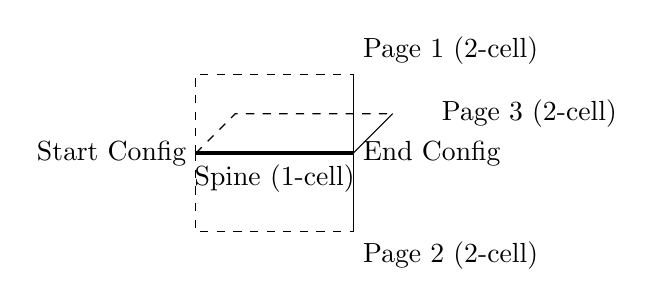
\begin{tikzpicture}
       % Define the spine (the 1-cell in Conf_n(Gamma))
    \coordinate (S1) at (0,0); % Start of spine (e.g., (v1, u2))
    \coordinate (S2) at (2,0); % End of spine (e.g., (v2, u2))

    % Draw the spine (making it thicker or distinct if desired)
    \draw[line width=1.5pt] (S1) -- (S2) node[midway, below] {Spine (1-cell)};

    % Define points for the "pages"
    % Page 1 (e.g., u2 -> u1 movement)
    \coordinate (P1_corner) at (2,1); % (v2, u1)
    \coordinate (P1_start_adj) at (0,1); % (v1, u1) -- optional, depending on how literal you want to be
    \draw (S2) -- (P1_corner);
    \draw[dashed] (S1) -- (P1_start_adj) -- (P1_corner); % Illustrate the 2-cell

    % Page 2 (e.g., u2 -> u3 movement)
    \coordinate (P2_corner) at (2, -1); % (v2, u3)
    \coordinate (P2_start_adj) at (0, -1); % (v1, u3)
    \draw (S2) -- (P2_corner);
    \draw[dashed] (S1) -- (P2_start_adj) -- (P2_corner); % Illustrate the 2-cell

    % Page 3 (e.g., u2 -> u4 movement)
    % This page will be "behind" or "in front" to show 3D effect
    \coordinate (P3_corner) at (2.5, 0.5); % (v2, u4)
    \coordinate (P3_start_adj) at (0.5, 0.5); % (v1, u4)
    \draw (S2) -- (P3_corner);
    \draw[dashed] (S1) -- (P3_start_adj) -- (P3_corner); % Illustrate the 2-cell

    % Add labels for conceptual understanding (optional, can be refined)
    \node[left] at (S1) {Start Config};
    \node[right] at (S2) {End Config};

    \node[above right] at (P1_corner) {Page 1 (2-cell)};
    \node[below right] at (P2_corner) {Page 2 (2-cell)};
    \node[above right, xshift=5mm, yshift=-3mm] at (P3_corner) {Page 3 (2-cell)};

    % Add some light shading to imply surfaces (optional)
    % This requires 'fill' and 'opacity', adjust as desired
    % \fill[blue!10, opacity=0.7] (S1) -- (S2) -- (P1_corner) -- (P1_start_adj) -- cycle;
    % \fill[green!10, opacity=0.7] (S1) -- (S2) -- (P2_corner) -- (P2_start_adj) -- cycle;
    % \fill[red!10, opacity=0.7] (S1) -- (S2) -- (P3_corner) -- (P3_start_adj) -- cycle;
 
\end{tikzpicture}
\caption{A three page book}
\label{fig:threepagebook}
\end{figure}
Pick any point on the spine of the book and take a small neighborhood \(U\).
% TODO, never say clearly
Clearly \(U\) is not homeomorphic to a surface.
Books are common structures found in configuration spaces.

